\section{背景}\label{sec:Background}

\subsection{基于 EVM 的区块链中的智能合约事件与交易日志}
智能合约通常由 Solidity~\cite{Solidity} 和 Vyper~\cite{Vyper} 等高级语言编写，并被编译为字节码，以便在以太坊虚拟机（Ethereum Virtual Machine，EVM）上执行~\cite{EVM}。基于 EVM 的区块链支持从简单转账到复杂 DApp 的广泛功能~\cite{DApp}。在这些区块链中，\textit{事件}和\textit{交易日志}实现了智能合约与外部系统之间的通信。当智能合约发出事件时，该事件会被记录为交易日志，其关键组成部分如下。

\paragraph{事件}
以 \texttt{Deposit} 为例，事件可被定义为一个元组 $E_{\texttt{Deposit}}(P_1, P_2, \ldots, P_n)$，其中参数 $P_i$ 可以是\textit{索引参数}（存储在\textit{主题}中），也可以是\textit{非索引参数}（存储在\textit{数据字段}中）。例如，在事件
\texttt{Deposit(address indexed account, uint256 amount, uint256 timestamp);}
中，\texttt{account} 是一个\textit{索引参数}，这意味着它会被包含在事件的主题中，从而使事件日志中的搜索和过滤更加高效。\texttt{amount} 和 \texttt{timestamp} 参数未被索引，但它们仍然提供了有关交易的重要信息。

%\liuye{Pls use detailed event declaration such as event Deposit(type indexed parameter, ...) to showcase. Otherwise, it is difficult for readers to understand what a event looks like, and what event topics and indexed parameters are.}

\paragraph{监听器}
监听器是指通过 RPC 方法订阅日志并监控特定事件的外部系统，例如 DApp 或钱包。

\paragraph{交易}
交易 $TX_{\textit{hash}}$ 表示区块链上的一次操作，例如调用智能合约中的函数 $f_{\texttt{name}}$。它包括发送方地址、接收方地址、转账金额，以及用于定义函数调用及其参数的输入数据。


\paragraph{发送者}
发送者 \( TX_{\textit{sender}} \) 是创建该交易的用户地址。

\paragraph{发出者}
发出者 $S_{\texttt{address}}$ 是在满足特定条件时触发事件的智能合约。

\paragraph{交易日志}
当智能合约执行过程中发出事件时，会生成日志 \( L_{hash} = (Topics_0^i, \allowbreak{} Data^i,\allowbreak{} S_{\texttt{address}}^i) \)。其中，\( Topics_0^i \) 表示第 \(i\) 条日志的事件签名，\( Data^i \) 包含非索引参数，\( S_{\texttt{address}}^i \) 是发出该事件的合约。这些日志存储在区块链上，并被用于事件监控。

%\liuye{Maybe we can have a unified definition for event log, e.g., event = (tx\_sender, emitter, event\_name, log\_data) and then detail each part. For me, I don't think we need to discuss much more about transaction log. We can briefly say like: a transaction may be associated with multiple event logs emitted by the called contracts. }

\subsection{代币}
在基于 EVM 的区块链中，代币以智能合约的形式实现，并遵循 \textit{ERC-20} 和 \textit{ERC-721} 等标准。这些标准定义了接口和事件，以确保不同 DApp 之间的兼容性。例如，ERC-20 规定了 \texttt{Transfer} 和 \texttt{Approval} 等事件，用于追踪代币转账和授权；而 \textit{ERC-721} 定义了类似事件，但适用于每个代币都具有唯一性的 NFT。这些标准化事件使钱包和交易所等外部系统能够监控代币活动，并实时更新用户余额或所有权记录，从而保证追踪的准确性和效率。

\begin{figure}[t]
    \centering
    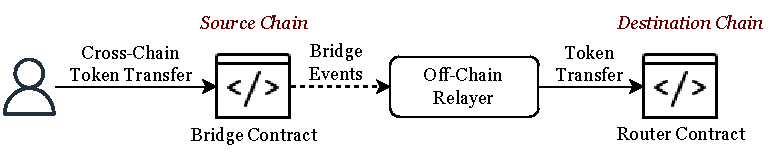
\includegraphics[width=\linewidth]{Sections/Picture/bridge.pdf}
    \caption{跨链桥的基本架构。}
    \label{fig:Bridge}
\end{figure}

\subsection{跨链桥}
一些 DApp 依赖链下模块来监控智能合约发出的交易和事件，以便实时获知链上活动和状态变化。例如，跨链桥会利用这些事件触发链下流程、更新用户界面或执行其他操作。

以跨链桥为例，如\cref{fig:Bridge}所示，\emph{源链}上的智能合约作为发出者 $S_{source}$，会在用户存入资产时发出 \texttt{Deposit} 等特定事件。而\emph{目标链}上的智能合约则作为执行方，由链下中继器调用，用于处理已存入的资产并完成转账操作。

当用户在源链上的\emph{桥合约}中存入代币时，会发出存款事件 $E_{\texttt{Deposit}}$，并将其记录为交易日志 $L_{deposit_{tx}}$。\emph{链下中继器}作为监听器，会监控这些日志以检测 \texttt{Deposit} 事件，处理事件信息，并与目标链上的智能合约协同完成资产转移。
